\section{Problem setup}
\label{sec:model}

\begin{figure}[t]
  \begin{centering}
  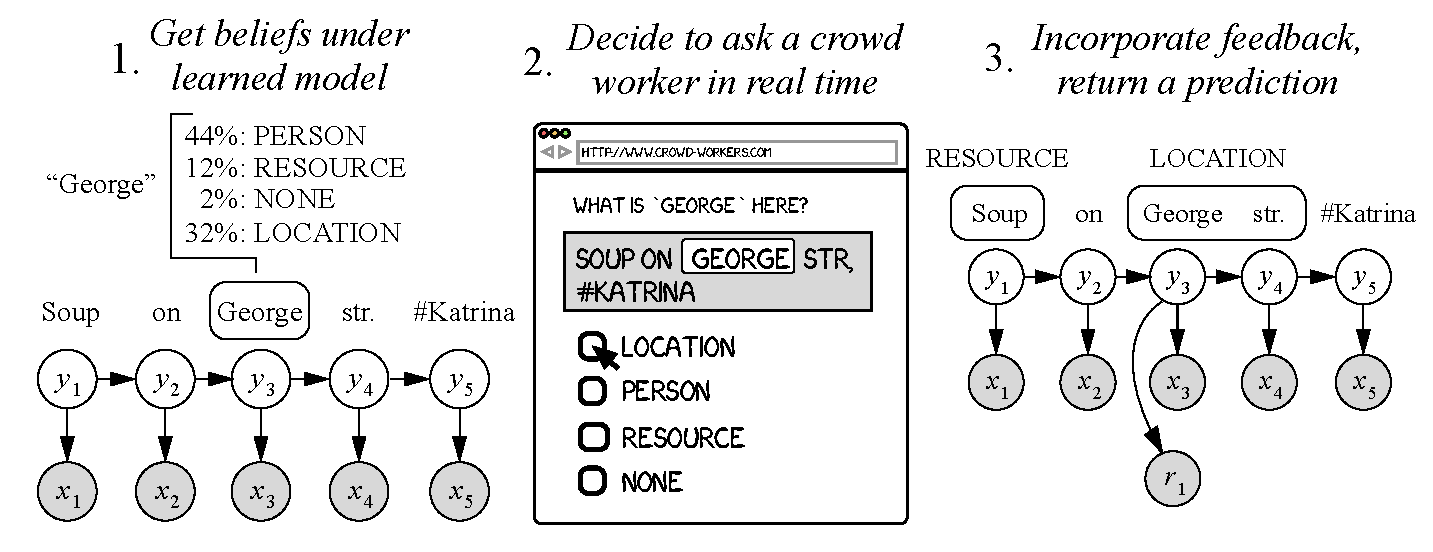
\includegraphics[width=1.0\textwidth]{figures/intro-banner.pdf}
  \end{centering}
  \caption{
    \pl{change $z_1$ to $r_1$}
    \pl{actually draw a CRF: there should only be nodes for $y_1, \dots, y_5$;
    the $x$'s should be technically one node, but you can just ignore it}
    Named entity recognition on tweets in on-the-job training.
    %(1) The system first runs a
%pre-trained model, discovers that the token ``George'' is ambiguous, and then
%asks a human for a label. The human label is returned in a few seconds,
%incorporated into the model, and the model then decides it has enough
%information to turn in a classification.
}
\label{fig:crf}
\end{figure}

\begin{figure}[t]
  \begin{centering}
  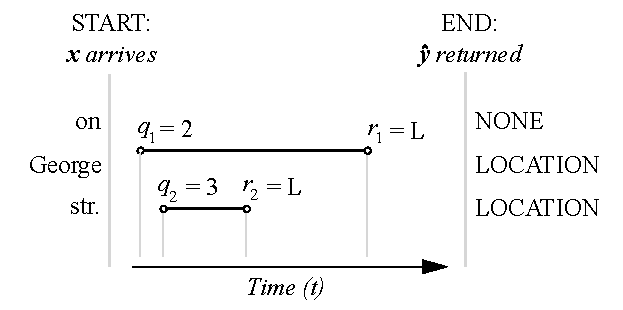
\includegraphics[width=0.49\textwidth]{figures/piano-roll.pdf}
  \hfill
 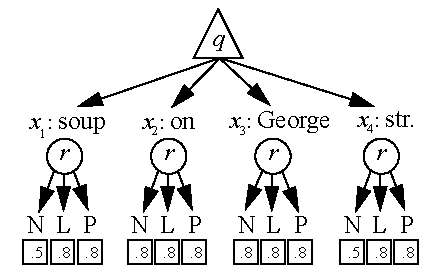
\includegraphics[width=0.49\textwidth,height=0.23\textheight,keepaspectratio]{figures/single-move.pdf}
  \end{centering}
  \caption{
    \pl{no '$\dots$', since $q_1 = 2$ has to refer to second position}
    \pl{maybe switch all examples to 'on George str.' or some other
    3 word phrase}
  }
\label{fig:piano-roll}
\end{figure}

% PL: need to define the task!
Consider a structured prediction problem from input $\bx = (x_1, \dots, x_n)$ to output $\by = (y_1, \dots, y_n)$.
For example, for named-entity recognition on tweets,
$\bx$ is a sequence of words in the tweet (e.g., \nl{on George str.})
and $\by$ is the corresponding sequence of tags (e.g., \scnone{} \scloc{} \scloc{}).
The full set of tags of \scper{}, \scloc{}, \scres{}, and \scnone{}.

In the \emph{on-the-job training} setting,
inputs arrive in a stream.  On each input $\bx$,
we can issue queries $q_1, q_2, \dots$ to the crowd to obtain tags (potentially more than once)
for any subset of the positions in $\bx$.
The responses $r_1, r_2, \dots$ come back asynchronously,
which are incorporated into the model.
\figureref{piano-roll}(left) shows one possible outcome:
we first query position $q_1 = 2$ (\nl{George}), which later returns $r_1 = \scloc$.
When we have sufficient confidence, we return the most likely prediction $\hat \by$.
We must make a prediction on each example,
and we are evaluated on accuracy $\text{acc}(\by, \hat\by)$
against the true tag sequence $\by$.
Note that $\by$ is never observed; the only feedback is via the responses.
In addition, this feedback is used to update the model.
Each query $q_i$ is also associated with a time $t_i$ between query and response
and an amount of money $m_i$ that the query cost.
Our goal is to choose the queries, maximize accuracy, minimize latency and cost.

%We receive a stream of inputs $\bx\oft1, \bx\oft2, \ldots, \bx\oft N$ with corresponding {\em unobserved\/} true output $\by\oft1, \by\oft2, \ldots, \by\oft N$ that we would like to predict.

% PL: too much detail about strategy
% at this point, just the get dynamics of the environment set up.
%Let us make our problem setting concrete with an example, depicted in \figureref{piano-roll}.
%We receive an input ``Soup on George str \#Katrina'' ($\bx$) and must produce
%an output ($\byt$) that labels words with the tags.
%Initially, our model is uncertain about both ``George'' and ``str''.
%We first query the crowd for a label on ``George'' ($q_1$) and then for a label on ``str'' ($q_2$). 
%After some time, the crowd responds with the label \scloc{} on both ``George'' ($r_1$) and ``str'' ($r_2$).
%At this point, the model is confident in its labeling, and we can turn in its
%prediction $\byt$.
%By querying the crowd queries $\bq = (q_1, q_2)$, we are not only able to
%produce a more accurate output, but can also use the responses $\br = (r_1,
%r_2)$ to train a better model.

%Of course, querying the crowd also incurs a cost for the queries as well as a
%time delay, $t$: $C(\bq, t)$ \pl{give example numbers that we used}

%In general, we want to maximize our accuracy by making queries while trading
%off the cost and time delay introduced.

% We cast this problem in the Bayesian decision theoretic framework: our objective is to maximize our expected utility under our current model,
% $\p(\by \given \bx, \br)$:
% \begin{align*}
%   u &= \E_{\by \sim \p(\cdot \given \bx, \br)}[1 - \ell(\by, \byt) + C(\bq, t)].
% \end{align*}

%\ac{Probably should talk more about training.} % PL: not really

%We receive a stream of inputs $\bx\oft1, \bx\oft2, \ldots, \bx\oft N$ with corresponding {\em unobserved\/} true output $\by\oft1, \by\oft2, \ldots, \by\oft N$ that we would like to predict.
%For each input $\bx$, we may query the crowd several times. Let $Q = \{q_1, \ldots, q_m\}$ be the set of queries.
%Finally, we observe responses $R = \{r_1, \ldots r_m\}$ to our queries after some time $t$.
%Using the information from these queries, our model makes the prediction, $\byt\oft{t}$.
%Our goal is to maximize the accuracy, trading off cost and latency as specified by a given objective function.
%
%More formally, suppose the output $\by\oft{t}$ has $n$ parts: $\by\oft{t} = y\oft{t}_1, \dots, y\oft{t}_n$.
%Let $q\oft{t} \in \{1, \ldots, n\}$ be a request for the label $y\oft{t}_q$,
%let $Q\oft{t} = (q\oft{t}_1, \dots, q\oft{t}_m)$ be a sequence of queries made on the $t$-th input and
%let $\tau\oft{t}$ be the time taken to make the prediction $\byt\oft{t}$. 
%We would like to minimize the cumulative loss, 
%following objective:
%\begin{align}
%  \sL &= \sum_{t=1}^T \ell_{\rmclass}(\by\oft{t}, \byt\oft{t}) + C(Q\oft{t}, \tau\oft{t}), \label{eqn:objective}
%\end{align}
%where $\ell_{\rmclass}$ is a given misclassification loss function, e.g.\ the Hamming loss, and $C$ is a given cost function.
%\ac{Concern: by using the cumulative loss, is there an expectation that we will ``model'' input and optimize for the future?}
%
%We now describe our choice of models for prediction, human error and latencies and return to optimizing \equationref{objective} in \sectionref{async}.
%
